\chapter{Background on Smartphones}
\label{chap:background}

In this chapter we introduce the architecture of modern smartphones with regard to both their hardware and software, as well as the mechanisms used to deploy applications onto them. Due to the amount of sensitive private data stored on smartphones, specific security measures have been implemented by vendors. In particular, smartphone vendors have implemented security mechanisms aimed at preventing malicious software from running on their operating systems or controlling what potentially malicious applications can do. These mechanisms have so far limited widespread malware infections that, in contrast, have plagued personal computers for decades. Additional mechanisms provide a way for users to manage which applications have access to which components and services of their smartphones. This form of control allows careful users to protect their privacy by choosing which private information to share with whom and which applications have access to restricted system components (e.g., access to the microphone, or to the pictures taken with the camera).

We note that different hardware and software vendors introduce slight variations into the basic concepts described in this chapter. While keeping the descriptions generic we will also highlight some differentiation factors between smartphone vendors. We will try to give an as up-to-date as possible view of the different system components. In this fast-evolving market, hardware and software vendors keep on increasing the security mechanisms used in their smartphones and in the whole ecosystem around them. Finally, we will focus our attention only on Android and iOS smartphones, the most used platforms in the current market (accounting to approximately 97\% of the global marketshare~\cite{marketshare}). Other popular smartphone platforms provide similar security architectures and mechanisms (i.e., Microsoft WindowsPhone~\cite{windowssecurity} and RIM's Blackberry~\cite{blackberrysecurity}).

Overall we try to present the reader with details that are of interest to the rest of this thesis and will help in understanding the following research chapters. The rest of this chapter is structured as follows, we first present the typical hardware architecture of a modern smartphone in Section~\ref{sec:bg_hardware}. We will see how we exploit some of the hardware components of smartphones in the first part of this thesis, where we use smartphones to secure our daily operations. We then introduce the different software components and highlight the security mechanisms provided by the operating system in Section~\ref{sec:bg_software}. Finally, we provide an overview of the two main distribution strategies for applications for Android and iOS devices in Section~\ref{sec:bg_markets}. In the second part of this thesis we will understand how attackers can overcome the security mechanisms implemented on current smartphones to carry out sophisticated attacks to steal users' credentials or private data.

\section{Smartphone Hardware}
\label{sec:bg_hardware}

A standard mobile device architecture (as shown in Figure~\ref{fig:bg_mobile})
has two processors. The \emph{application processor} runs the mobile OS (e.g.,
Android) and the applications on top of it. The vast majority of devices
use ARM as the architecture for their processors. This is due, mainly, to
ARM cores small footprint and reduced power consumption while offering powerful
multi-core options. Modern ARM processors, from ARMv7 onwards,
typically support both the ARM and the Thumb-2 instruction
sets~\cite{arminstructionset}. The original iPhone, in 2007, was one of the first smartphones to use an ARM processing core. Ever since, the majority of modern smartphones have used ARM cores as their main processing unit. The more recent ARM cores (since ARMv6) also support a system-wide security mechanism called ARM TrustZone. We defer the discussion on ARM TrustZone to Section~\ref{sec:ps_tee_mobile} as it will be the focus of that research chapter.

\begin{figure}[!ht]
    \centering
    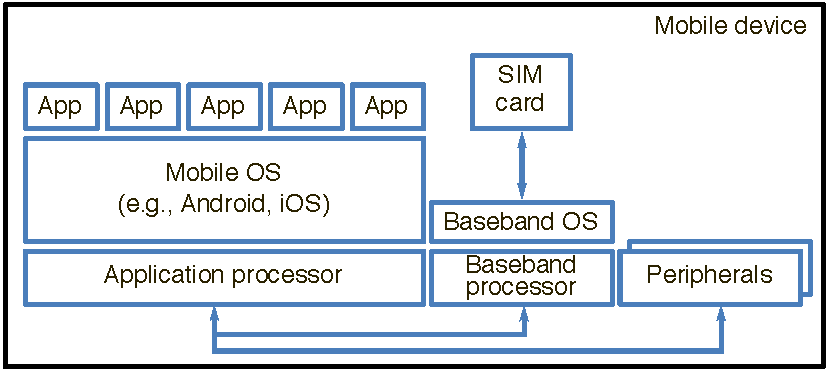
\includegraphics[width=.9\linewidth]{figures/others/bg_smartphone}
    \caption[Architecture overview of a modern smartphone]{Architecture overview of a modern smartphone. The application processor is separated from the baseband processor that handles network operations and communicates with the SIM card. Applications run on top of a mobile operating system (e.g., Android or iOS).}
    \label{fig:bg_mobile}
\end{figure}

The mobile OS that runs on the application processor has direct access to the
peripherals found on the device and mediates this access to the unprivileged
applications running on top. A common set of peripherals found on modern
smartphones consists of a wireless adapter (implementing both WiFi as well as
Bluetooth functionality, such as the Broadcom BCM4354~\cite{broadcombcm}), a
GPS receiver (such as the Broadcom BCM47521~\cite{broadcomgps}), one or more
gyroscopes and accelerometers (such as the InvenSense's
ICM-20608-G~\cite{6axis}), one or two integrated cameras, and a set of
microphones and speakers. A physical keyboard and pointing device are typically
omitted and a software-based implementation that shows on the screen is
preferred. This plethora of peripherals is one feature that distinguishes
smartphones from other mobile devices and personal computers and enables many
different applications, some of which malicious, as well as some interesting
security solutions.

A \emph{baseband processor}, running the baseband OS, handles cellular
communication and mediates communication between the application processor and
the SIM card. Each SIM card has a unique identifier called IMSI (International
Mobile Subscriber Identity), used to negotiate with a base station to grant
access to the mobile network. The baseband OS is the responsible for
implementing the protocols that govern the mobile networking space. For
example, it must implement the stacks used for GSM~\cite{etsigsm},
GPRS~\cite{etsigprs}, EDGE~\cite{etsiedge}, LTE~\cite{etsilte}. The
application processor and the baseband processor interact by exchanging
messages, typically through a shared memory region. Device manufacturers are
free to integrate any baseband OS of their choosing. Typically such operating
systems are small microkernel-based real-time operating systems customized for
baseband processors. Notable examples are: Nucleus RTOS~\cite{nucleos},
ThreadX~\cite{threadx} and OKL4~\cite{okl4}. Due to the fact that baseband OSs are interfacing directly with the network providers and that they have full access to the smartphone hardware, they are typically well tested and undergo
strict code audits to ensure that they are free of bugs. While some attacks against baseband processors have been found~\cite{basebandwoot,basebandccc}, their numbers are relatively small compared to bugs found in more complex operating systems.

\section{Smartphone Software}
\label{sec:bg_software}

We now briefly describe the software architecture of Android and iOS operating systems. We then focus on their security features. We first introduce the features generically and then focus on more details for the Android OS, which is also used in the rest of this thesis as the main smartphone OS for discussion.

Smartphone operating systems are based on a monolithic kernel, such as the
Linux kernel~\cite{androidkernel} (for Android) or a hybrid kernel such as
Mach~\cite{machkernel} (for iOS). The kernel implements common functionality
(such as process and memory management, filesystem access, drivers to access
the peripherals). On top of the kernel, the OS features a layer of software
that is both the foundation for developers to develop their applications (so
called Software Development Kits, or SDKs) as well as a set of pre-installed
privileged utilities to manage the system. Examples of these utilities are a
network manager, a way to configure the many preferences of the system, a
centralized notification center, and so on. The development framework dictates
the running environment as well as the main development language of the
operating system. Finally, a number of applications come bundled with the OS.
Examples include an internet browser (on iOS an offspring of Safari, based on WebKit~\cite{webkit}, and on Android a mobile version of Chrome, based on Blink~\cite{blink}), an e-mail client, a calendar application, an address book application, and so on.

We now introduce how third party applications can be developed on both Android and iOS and then focus our attention on the security features provided by both architectures.

\subsubsection*{Android Application Development}

\begin{figure}[!t]
    \centering
    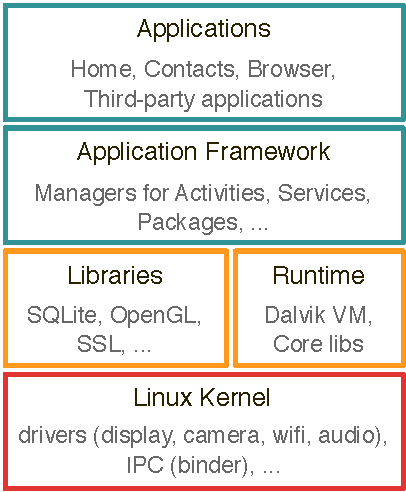
\includegraphics[width=.5\columnwidth]{figures/others/bg_android}
    \caption[Android software components]{Android software components. The Linux kernel sits at the lowest level and manages drivers and other OS components. The runtime environment runs Dalvik executables, which can interface with system libraries. The application framework allows applications to use standard components such as activities and services. Finally, on top, applications are the front end to the user.}
    \label{fig:bg_android_stack}
\end{figure}

Android applications are Dalvik executables~\cite{dalvik}, where Dalvik is a
small implementation of Java specifically tailored for ARM processors and
optimized for mobile platforms. Each application is developed in a type-safe
language very similar to Java, and is run in a virtual machine (the so-called
ART: Android runtime). Developers can also develop applications in C or C++ by
using the Android NDK (Native Development Kit) and providing an
interface to communicate data back and forth with the Dalvik application.
Developing against the NDK allows for fast ARM-optimized code and also allows
developers to use any C/C++ library, like opengl~\cite{androidopengl}, or
ProjectNe10~\cite{projectne10} used to access ARM Neon optimized routines.
Figure~\ref{fig:bg_android_stack} shows an overview of the main software
components of an Android device.

Applications are developed using a set of Dalvik classes and XML files which define a plethora of parameters (e.g., string values, localization information, color combinations) as well as GUI descriptions. These values are either compiled in the application at compilation time or parsed at runtime by the OS to, for example, draw the GUI of the application on the screen. Developers can also draw GUI elements programmatically. Applications can have a number of components, and, most notably, can be split into \emph{Activities}, the foreground processes that interact with the user, and \emph{Services}, the background processes that can be used to perform long running operations or are active when an application goes into background. The system, indeed, allows background applications to perform any kind of task, like monitoring the GPS coordinates, record sound through the microphone and perform any network activity. 
% Figure~\ref{fig:bg_android_lifecycle} illustrates the lifecycle of an Android application for both its activities and services, which can continue to run in the background once the main Activity loses the foreground.

% \begin{figure}[!ht]
%     \centering
%     \subfigure[] {
%     \includegraphics[width=.45\columnwidth]{figures/others/bg_android_activity_lifecycle}}
%     \subfigure[] {
%     \includegraphics[width=.45\columnwidth]{figures/others/bg_android_service_lifecycle}}
%     \caption[Android applications lifecycle]{Android applications lifecycle for an Activity (a) and a Service (b). In particular we see that applications are composed of multiple Activities and Services which can continue to run even when the application enters a background state.\todo{new images}}
%     \label{fig:bg_android_lifecycle}
% \end{figure}

We refer the interested reader to the Android developer portal for a complete overview of Android system components, development practices and possible applications~\cite{androidkernel}.

\subsubsection*{Apple iOS Application Development}

iOS applications are compiled binaries implemented in Objective-C, an
object-oriented dialect of C. Starting with iOS 7, applications can also be
developed in Swift, a new open-source object-oriented language developed by Apple~\cite{swift}. Through Objective-C glue code applications are able
to directly use C/C++ libraries and have direct access to ARM functions through
the direct use of assembly code. Developers make extensive use of the CocoaTouch
runtime framework to interact with system components and the user interface. The latter can be implemented either programmatically or
through XML-based files. Figure~\ref{fig:bg_ios_stack} shows an overview of the
main software components of an iOS device.

\begin{figure}[!t]
    \centering
    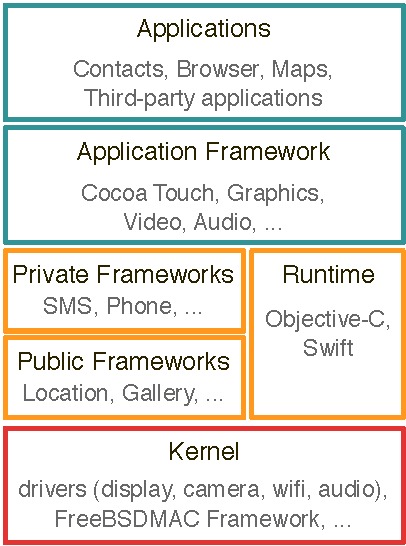
\includegraphics[width=.5\columnwidth]{figures/others/bg_ios}
    \caption[iOS software components]{iOS software components. The kernel is at the lowest level and manages drivers, OS components and the security mechanisms. The runtime environment runs Objective-C and Swift applications. Applications can use the public libraries and the application framework components.}
    \label{fig:bg_ios_stack}
\end{figure}

In contrast to Android applications, iOS applications are monolithic. In order to run longer-running tasks, each process can spawn multiple threads. The application lifecycle is also different from Android's in that, once in the background, applications are typically fully suspended or can continue to operate for a finite period of time (a number of seconds or minutes, at most), mostly in order to preserve battery life. A handful of exceptions to this rule are applications that require GPS updates (e.g., a mapping application or an activity logger), perform VoIP functionality (e.g., Skype) or play music (e.g., Spotify). With the recent release of iOS 9, Apple allows for two applications to run concurrently on some devices (e.g., the iPad Air 2, the iPad Pro and the iPad mini 4) and for both to display content on the screen. Apart from when they are in the foreground, applications can execute arbitrary code only upon receiving a \emph{silent} push notification. When this happens the application has approximately 30 seconds to, for example, fetch data from a server. 
% Figure~\ref{fig:bg_ios_lifecycle} illustrates the lifecycle of an iOS application.

% \begin{figure}[!ht]
%     \centering
%     \includegraphics[width=.8\columnwidth]{figures/others/bg_ios_lifecycle}
%     \caption[iOS applications lifecycle]{iOS applications lifecycle. In particular we see how applications are monolithic and enter a suspended state as they go into background.\todo{new image}}
%     \label{fig:bg_ios_lifecycle}
% \end{figure}

We refer the interested reader to the iOS developer portal for a complete overview of iOS system components, development practices and possible applications~\cite{iosdevelopment}.

\subsection{Security Features}

In terms of security, each OS features different mechanisms that we will now present in more detail.

\paragraph{Secure Boot.} Modern smartphones employ, in most cases, a standard
secure boot chain. Android manufacturers can develop their own version, with a
potentially slightly modified strucutre. Some enable a modified (and unsigned)
kernel to run right out of production (albeit typically voiding the phone
warranty), and others lock the platform and require hacks, so-called
\emph{device rooting}, before an unsigned kernel can be booted. Apple's iOS
devices, on the other hand, all follow the same procedure, which we now detail.
Upon device boot, the application processor runs code from the Boot ROM (a
read-only memory region burnt-in at hardware manufacturing time) which
consitutes the hardware root of trust. Apart from the boot code, the Boot ROM
also contains the Apple Root CA public key, which is used to verify the
integrity of the Low-Level Bootloader (LLB). The LLB, when it has finished
running its tasks, in turns verifies the integrity of the next bootloader
(iBoot) which finally verifies and boots the iOS kernel. For any unsigned
kernel to boot, the phone must be rooted. Exploits for each new kernel
version must be discovered in order for the modified kernel to be booted up
correctly. It is common that rooted devices modify the framework running on top
of the kernel (or some kernel extensions), rather than the kernel itself.

Similar to the application processor, the baseband processor and the code running in the trusted execution environment (if any) follow a similar procedure to make sure that the code that runs at the lowest level on a device is verified and has not been modified.

\paragraph{Application Sandboxing.} Each application running on top of the
operating system and developed using the system SDK is sandboxed in its own
execution environment. The sandbox makes sure that at runtime the application
cannot access code or data used by another application (memory isolation). In
Android, memory isolation is typically achieved by starting each application in
its own virtual machine. The system then performs two levels of access control
enforcement: \emph{(i)} the middleware component controls IPC calls and
\emph{(ii)} each application is assigned a locally unique Linux UID and the
kernel enforces access to low-level resources based on these. In contrast, iOS
performs memory isolation through the use of kernel-level process-based
isolation to protect the address space of each application and of other system
resources. Both platforms support address space layout randomization (ASLR), so
that memory regions are randomized at launch, both for system processes and
third party applications~\cite{androidsecurity,applesecurity}. Furthermore the
use of ARM's Execute Never (XN), which marks memory pages as non-executable
improves the overall memory protection. On iOS, only Apple-approved (and, to
the best of our knowledge, only Apple-developed) applications can overcome this
limitation to, for example, enable the JavaScript just-in-time compiler of the
system browser.

\paragraph{Storage Isolation.} Applications data integrity and confidentiality
is protected when at rest. On Android, each application is assigned its own
unique user identifier (Linux UID), as if it were a different user on the
system. Storage isolation is then implemented as file-system permissions.
Application files are created by default as owned by that particular user on
the system and are, hence, accessible only by it. An application can also
create world-readable and world-writable files that can then be accessed by any
other application. On systems that provide an external storage medium (e.g.,
smartphones that allow the user to expand the internal storage with an
SD-card), any data stored in the external storage can be accessed by any
application. This is mainly due to the fact that external storage is typically
formatted as FAT which does not support Unix access-control bits.

On both iOS and Android, third party applications can further store their data
in encrypted form through the use of special
APIs~\cite{applesecurity,androidsecurity} that make use of device-specific and
application-specific keys. On iOS devices the Data Protection framework
combines a device-specific key together with the user's passcode (i.e., either
a 4-digit PIN or a longer alpha-numeric password) to generate per-application
or per-file keys to keep stored data in an encrypted form. These operations
happen transparent to the developer aided by the OS as well as the hardware.
While an iOS application's data is stored in encrypted form automatically, on
Android devices the developers decide what to store encrypted and how. Android
provides a plethora of hardware-accelerated encryption routines available
through the Java API.

\paragraph{Permission-based Architecture.} Applications running on top of smartphone operating systems do not have direct access to peripherals or stored user's data. Instead, all access is mediated by the kernel, the operating system and the upper-layer framework. When mediating access to peripherals (such as the microphone, or the camera) as well as to data (such as contacts or GPS location) the OS performs access control checks to make sure that the application accessing the private information has indeed been granted access to it (what is called a permission). 

Android and iOS have a different approach to permissions. Android has roughly 138 permissions (at the time of this writing, for API level 21). For example, applications require permissions to access the internet, to read the contacts, to manipulate the pictures stored in the photogallery, or to receive location information. We refer the reader to the information available with Google for further details~\cite{androidsecurity}. In contrast, permissions on iOS devices are very coarse-grained. At this time, the system requires explicit permissions to access: the microphone, the camera, photos, location information, contacts, calendars and reminders, the motion activity sensor (on iPhone 5s and later), social media accounts, HomeKit and HealthKit and Bluetooth sharing~\cite{applesecurity}. Finally, the user has to explicitly allow applications to receive push notifications.

\begin{figure}[!t]
    \centering
    \subfigure[] {
    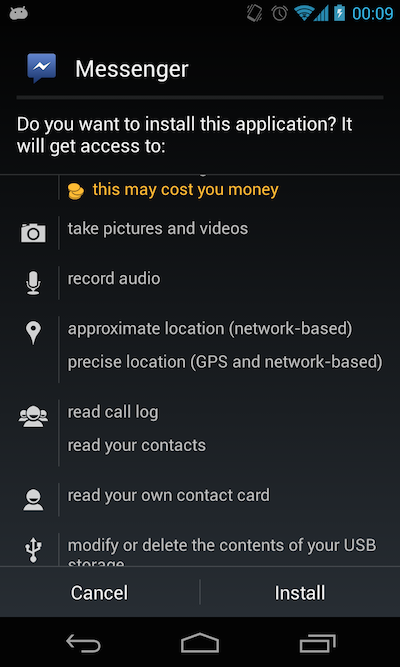
\includegraphics[height=220px]{figures/others/bg_android_permission}}
    \subfigure[] {
    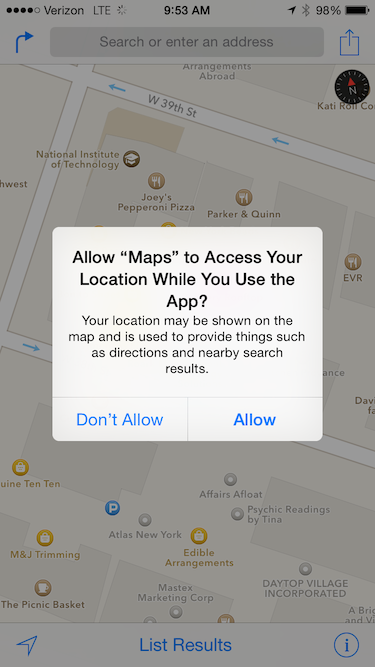
\includegraphics[height=220px]{figures/others/bg_ios_permission}}
    \caption[The permission dialog for both Android and iOS shown to the user]{The permission dialog for both Android version 4.3 (a) and iOS version 7 (b) shown to the user. On Android the dialogue appears at install time. If the user does not approve the required permissions the application is not installed. On iOS the user is prompted with a dialogue to allow the access to a specific resource at run-time.}
    \label{fig:bg_permissions}
\end{figure}

Permissions are further handled differently by the two platforms both from the developer as well as from the user's perspective. On Android, the developer has to specify in the application's \emph{manifest} file (which also specifies the application ID, name, and other details) all the permissions required by its application to run. The manifest is parsed on the marketplace to show to the user which permissions are required. Upon installation it is parsed by the Android OS to grant the correct set of permissions to the process. Up until Android 6.0, released in late 2015, users could only accept or deny (the latter resulting in the application not being installed) all the permissions required by a specific application at install time. In order to help users make sense of the potentially long list of permissions required by an application, the OS bundles fine-grained permissions into broader categories (as shown in Figure~\ref{fig:bg_permissions}~(a)). This mechanism has changed recently and users can now revoke previously granted permissions to an application by going in the system settings. On iOS devices, the developer does not have to specify permissions while developing the application. At run-time, the operating system blocks the first access to any protected resource and prompts the user with a system dialog to deny or grant access to the resource (as shown in Figure~\ref{fig:bg_permissions}~(b)). Again, the user is able to revoke a previously granted access to a resource by going into the system settings.

\paragraph{Application Signatures.} On both Android and iOS, applications are signed packages. On the Apple platform, only software signed by a valid Apple-issued certificate will be permitted to be installed and run. This mechanism extends the chain of trust to third-party applications and prevents unsigned code and self-modifying code from executing. Developers are required to sign their applications with an Apple-issued certificate that is released only after verification of the individual or organization requesting it. This allows Apple to bind each application with a particular identity, discouraging the creation and distribution of malicious code through their marketplace. All the signature checks are performed at runtime by the iOS kernel before starting an application. On Android, in contrast, applications can be signed with self-signed certificates that anyone can produce. In fact, the main reason behind signing applications on Android, is not to prevent unsigned code from running on the platform (which is possible), but rather to maintain a same-origin principle for application updates. On Android, it is possible to ship an update to an application only if said update is signed by the same key used for the previous version.

\paragraph{Trusted Execution Environments.} Smartphones have different Trusted Execution Environments (TEEs) available. In general, a TEE is any environment that is able to store secrets (e.g., private keys, passphrases) and run code in isolation from the main operating system. All smartphones have a SIM card, which can run small applets~\cite{global} (known, since before the advent of smartphones, as SIM applications). Such applets come pre-installed on the SIM card and have to be endorsed by the carrier operator in order to be deployed to customers' SIM cards. 

Another option to perform operations in a trusted environment is ARM TrustZone, which is available on ARM cores since the Cortex-A series~\cite{ARMTrustZone,armTZslides}. We will go into more detail on how ARM TrustZone works in Chapter~\ref{chap:ps_tee}. As an overview, a TrustZone-enabled device supports two execution modes whose isolation is controlled and enforced in hardware. The \emph{normal world} executes the main operating system (e.g., Android or iOS), while the \emph{secure world} executes a smaller, typically more secure, operating system (e.g., an L4-variation on Apple's iPhones~\cite{applesecurity}, or a custom Trustonic OS on some versions of the Samsung Galaxy family~\cite{trustonicknox}). On previous phones and earlier smartphones, the TrustZone technology was more tied down by the device manufacturer and used for SIM locks and similar features~\cite{kostiainen2011codaspy}. Although the software running in the secure world potentially has access to all resources of the device (unlike software running on SIM cards), one of the main design goals is to keep this software small and verifiable in order to prevent bugs in this higher-privilege execution mode.

Although some proposals have been made in order to allow third-party developers to tap into the potential of smartphone TEEs~\cite{kostiainen09asiaccs,kostiainen2011acns,kari11stc}, at the time of this writing the software in the secure world is mostly controlled by device manufacturers. Apple uses the secure world (the \emph{secure enclave}, in Apple's terminology) to store encryption keys and to perform fingerprint matching from its Touch ID peripheral. Samsung proposed their KNOX platform~\cite{trustonicknox} to enable businesses to store credentials and encryption keys in the secure world of TrustZone-enabled devices.

\paragraph{Secure Peripherals.} Starting with the iPhone 5S and on some Android models (e.g., the Samsung Galaxy S5) hardware manufacturers have started to embed secure peripherals. By secure peripherals we mean peripherals that are not accessible from applications directly. For example a fingerprint reader that both provides added security to the device as well as is securely integrated with the rest of the hardware. In this space, Apple's Touch ID stores the scanned image(s) into the encrypted memory of the secure enclave and the memory region is wiped as soon as the Touch ID sensor is deactivated. Only software running in the secure enclave is able to process the scanned copies of the fingerprint which are never accessible from the rest of the system. While fingerprint-based access (and, in general biometric-based access control) is prone to false positives and negatives and can be circumvented~\cite{cccfingerprint}, the intention is to force users to enable passcodes on their phones, which in turns enables stronger secure storage. The general idea being that a larger population using a passcode (and more people using stronger passcodes, since they are required to type them in less frequently) is better than leaving devices unprotected for longer periods of time or missing a passcode altogether.

\section{Distribution Markets}
\label{sec:bg_markets}

Smartphone vendors have adopted a controlled system to let users install third-party applications in the form of \emph{marketplaces}. Apple's AppStore~\cite{appstore} and Google Play~\cite{googleplay} are the most secure way (and in the case of Apple the only way) to install applications on a smartphone. This distribution model has some security advantages which we now outline in brief.

First of all, applications developed by third parties are submitted to the marketplaces and vetted before publication. Apple has a tight control model in which applications are subjected to static and dynamic analysis to check that they do not contain any potentially malicious code or that they use undocumented or private APIs. Then they are tested by a team of people to make sure that applications conform to visual guidelines but also to test for obvious bugs or problems created by each application. The whole testing procedure takes between one and two weeks in most cases, and terminates with the application being prepared for download by customers or being rejected with some motivation. The Android market follows a similar procedure, although applications tend to be published more quickly. Static and dynamic analysis (there is evidence that applications are tested in an emulator~\cite{googlebouncer,bouncerdissect}) is performed in the background and the application is pulled from the market should anything malicious be detected. Although these mechanisms do not fully prevent malware from making its way to a large number of customers, they are providing a first line of defense against malware. In fact it is observed that the amount of malware present on smartphones is significantly smaller, compared to other (more open) systems~\cite{lever-ndss13,truong13}.

Second, the marketplace managers (i.e., Apple and Google, although smaller ones exist such as from Amazon~\cite{amazonappstore}), that have all applications in a single repository can perform large-scale analysis to detect potentially malicious applications. This has, for example, led to the discovery of some malware masquerading as legitimate banking applications and trying to steal user credentials~\cite{droid09}.

Another security advantage of the distribution model of smartphone applications is that it allows for continous and fast upgrades. This is true for third-party applications that can be updated (potentially fixing security bugs) and that will in turn be automatically downloaded and installed by the majority of the user base (this option is typically on by default but could be switched off, if desired by the user). Similarly, OS (and firmware) software updates are enabled over-the-air (OTA), something that again makes adoption of security fixes fast. For example, at the time of this writing, the iOS 8 (introduced in September 2014) adoption rate is 41\% and iOS 9 (introduced in September 2015) is at 52\%. On Android the numbers are lower, due to a more varied landscape in terms of devices: Android 4.4 (introduced in October 2013) is at 39\%, Android 5.0 (introduced in November 2014) is at 21\%.\footnote{The most up-to-date numbers can be found at \url{https://developer.apple.com/support/app-store/} for Apple devices and at \url{https://developer.android.com/about/dashboards/index.html} for Android devices.}

Finally, applications installed through marketplaces can be remotely removed from devices or disabled in case malicious activity is detected. Although some consider this activity a violation of user's privacy (the act of remotely disabling applications), it is also a strong security mechanism in case malicious software indeed finds its way through to users.

\paragraph{Sideloading.} Although installation of applications through marketplaces is the recommended and typical way for users to install software on their smartphones, on Android it is also possible to install unsigned software from other places. This operation, known as sideloading, is potentially an attack vector.

On Apple devices it is not possible to install any third party application unless it is signed and comes from the AppStore. The only possibility to install and run unsigned content is to root or jailbreak the one's device. This operation disables the security checks performed by the operating system at runtime and hence, similar to Android, is a potential security risk for end users.

\section{Summary}

We have given a broad overview of smartphone platforms both in terms of hardware and software. In particular, after a generic introduction, we focused on the details that will be most useful to better appreciate the rest of this thesis. We will see how the hardware configurations of current smartphones enable solutions where they are used as an effective and usable two-factor authentication mechanism for daily operations. The second part of this thesis will focus on the software security mechanisms deployed today by device vendors and how they can be circumvented to steal users' private data.


